\documentclass{article}
\usepackage[utf8]{inputenc}
\usepackage{subfigure}
\usepackage{float}
\usepackage{graphicx,xurl}
\usepackage{amsmath,amsfonts,amsthm,amssymb,bm,bbm}

\title{Properties of WATG in $H \times C$ plane}
\author{Eduarda Chagas}

\begin{document}

\maketitle

In this report, we present experiments to analyze the response of WATG to different noise levels.
Our truth is the deterministic image generated by the function:
\begin{equation*}
z(x,y) = \sin (4x + 0.5y), 
\end{equation*}
where  $x, y \in [-2\pi, 2\pi]$.

The speckle noise was modeled as outcomes of independent, identically distributed unitary-mean Gamma random variables with shape parameter $L$ (the number of looks, which controls the signal-to-noise ratio)
$W(L) \sim \Gamma(L, L)$,
with $L \in \{1, 100, 150, 200, 250, 300, 350, 400, 450, 500\}$.
The observed images $I(L)$ are the pixelwise product of $z$ and $w(L)$.

Thus, here we analyzed the effect of see $I(L) = m_\alpha (z) \cdot W(L)$, where $m_\alpha$ is the function that maps $[0,1]\mapsto [\alpha,1]$.
Two experiments were conducted:
\begin{enumerate}
    \item Analysis of the variation of texture $I$ in $H \times C$ Plane when we keep $\alpha$ fixed and we vary $L$, and
    \item Analysis of the variation of texture $I$ in $H \times C$ Plane when we vary $\alpha$ and keep the number of $L$ fixed.
\end{enumerate}

As we can see in Fig.~\ref{Fig:TestA}, and Fig.~\ref{Fig:TestL}, in both cases, variations in the rescaling factor do not affect the deterministic structure of the texture, maintaining the maximum statistical complexity and increasing its entropy.

\begin{figure}[H]
	\centering
	\subfigure[$I(100)$]{\label{Fig:TestL100}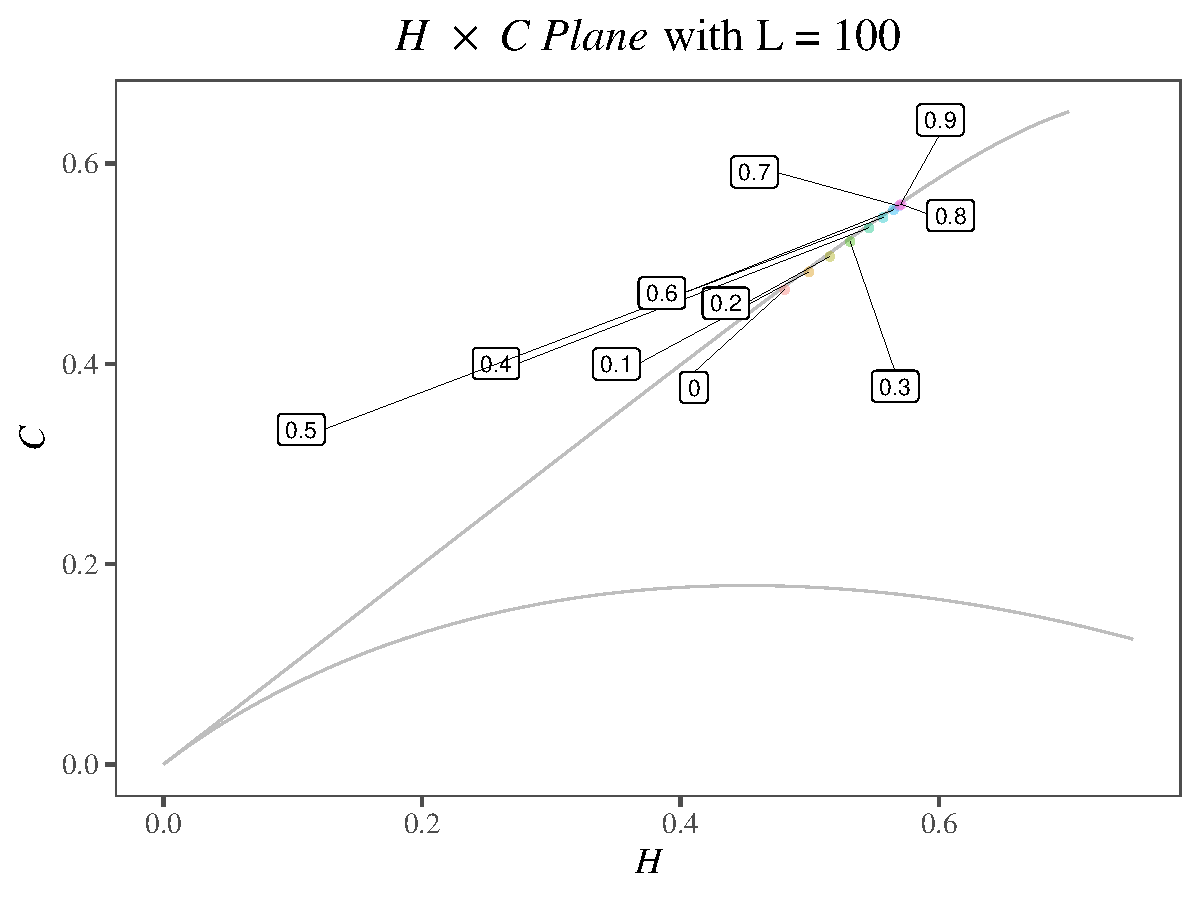
\includegraphics[width = 39mm]{p_L100.pdf}}
	\subfigure[$I(300)$]{\label{Fig:TestL300}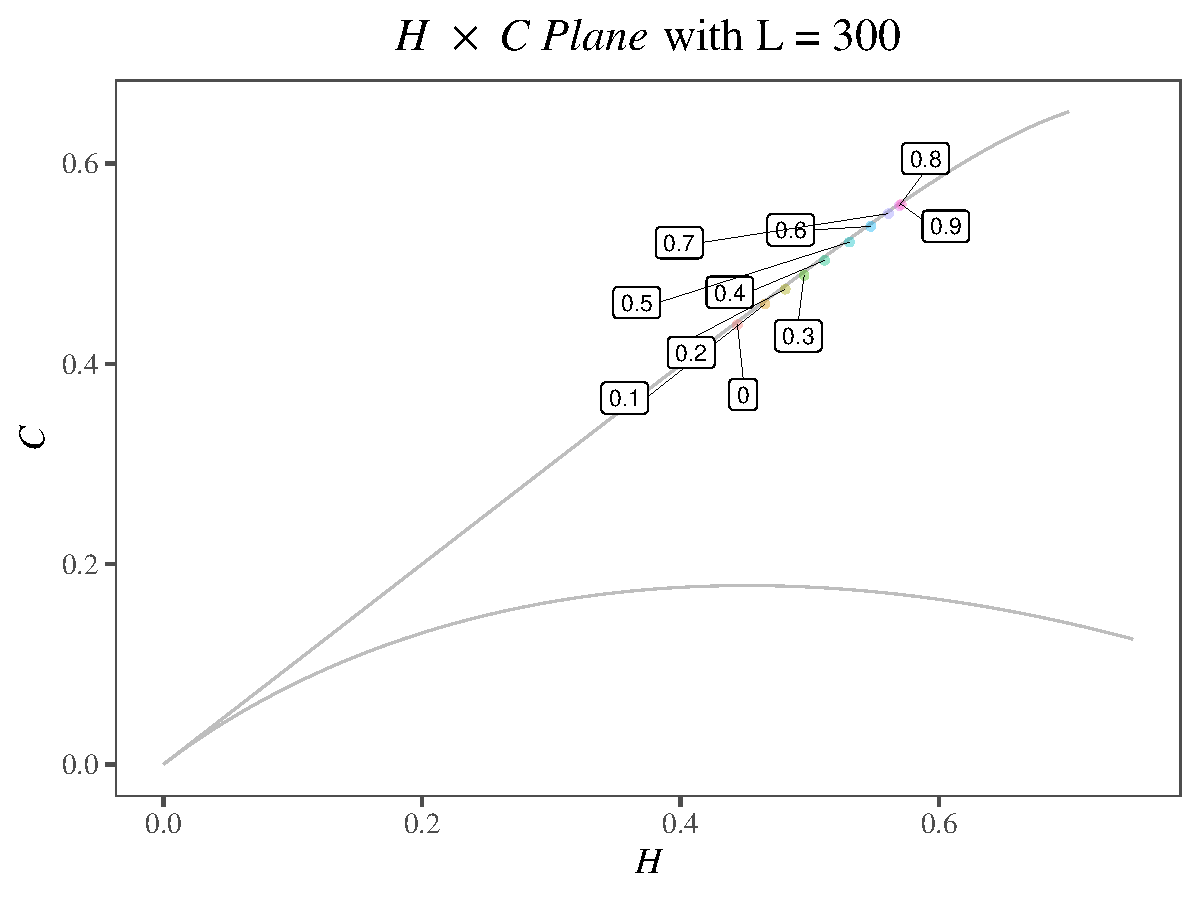
\includegraphics[width = 39mm]{p_L300.pdf}}
	\subfigure[$I(500)$]{\label{Fig:TestL500}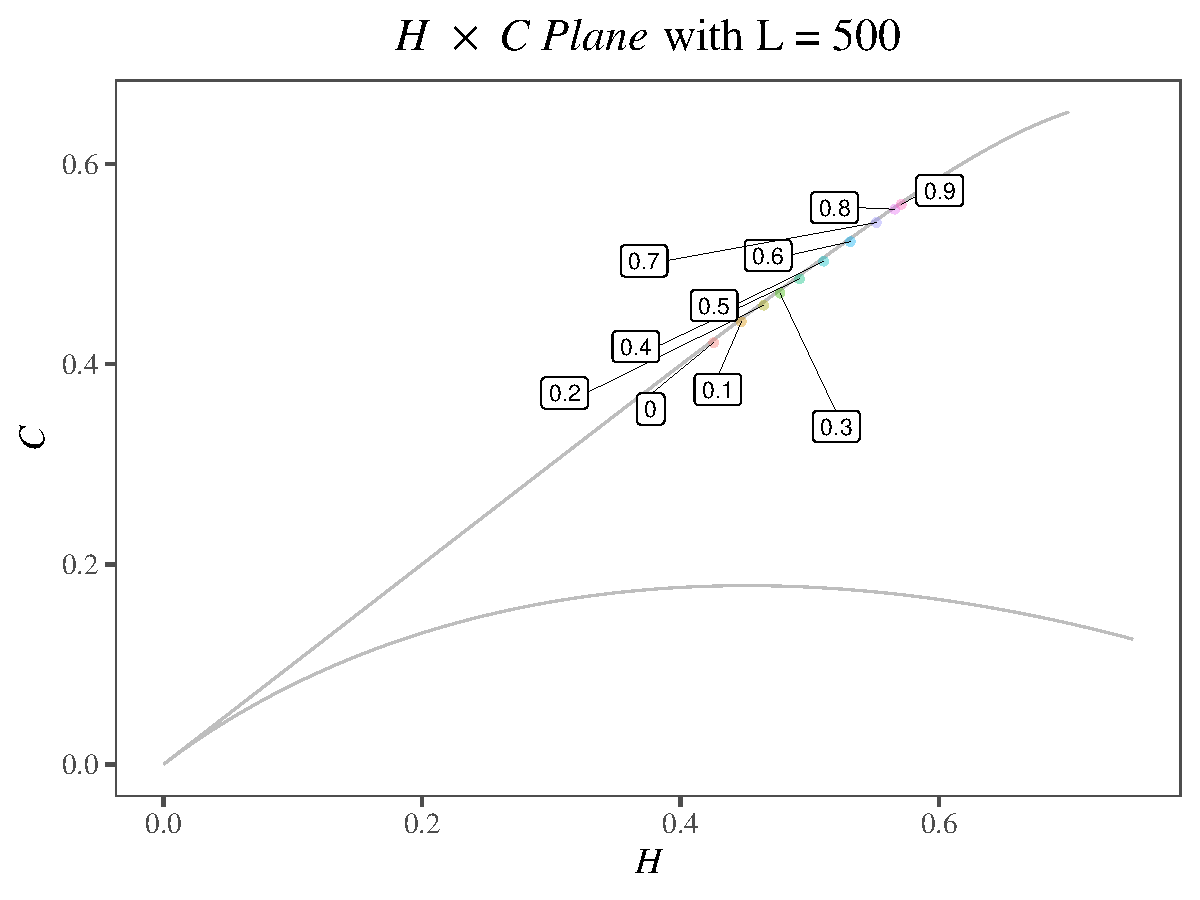
\includegraphics[width = 39mm]{p_L500.pdf}}
	\caption{Analysis of deterministic image varying $\alpha$.}
	\label{Fig:TestL}
\end{figure}

\begin{figure}[H]
	\centering
	\subfigure[$\alpha = 0.5$]{\label{Fig:TestA.5}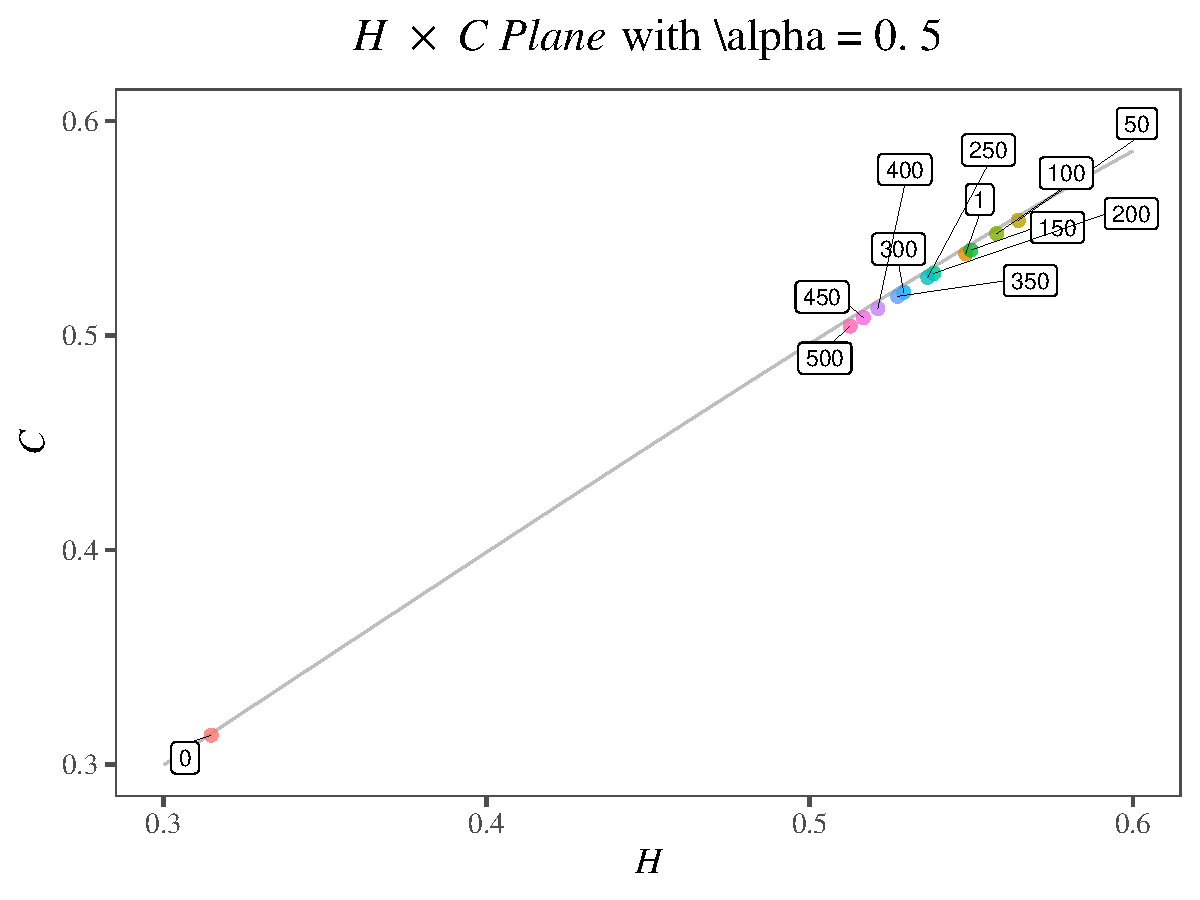
\includegraphics[width = 59mm]{p_a.5.pdf}}
	\subfigure[$\alpha = 0.5$]{\label{Fig:TestA.9}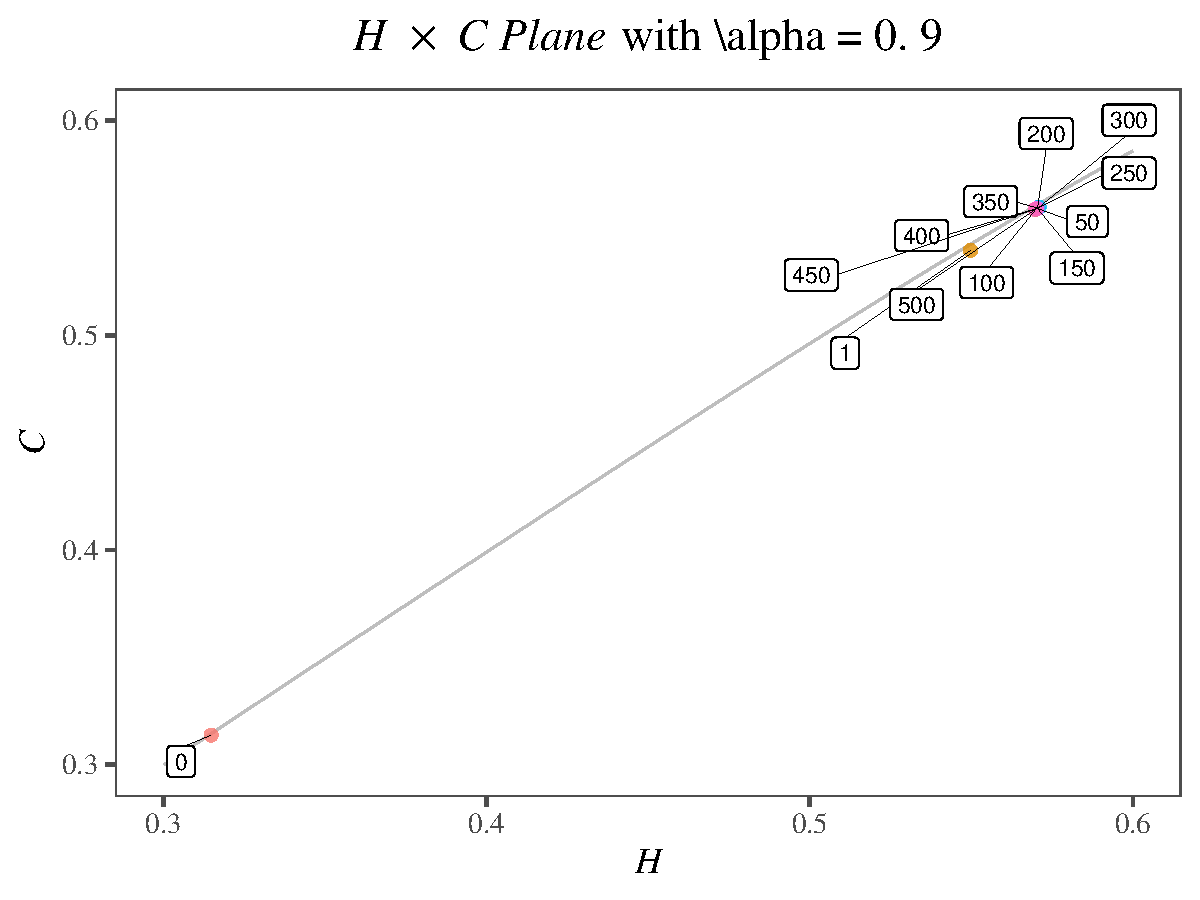
\includegraphics[width = 59mm]{p_a.9.pdf}}
	\caption{Analysis of deterministic image varying $L$.}
	\label{Fig:TestA}
\end{figure}

\end{document}
